\printconcepts
\exercise{Name two different things that cannot be described with just one number, but rather need 2 or more numbers to fully describe them.
}{Answers will vary.
}

\exercise{What is the difference between $(1,2)$ and $\la 1,2\ra$?
}{$(1,2)$ is a point; $\la 1,2\ra$ is a vector that describes a displacement of 1 unit in the $x$-direction and 2 units in the $y$-direction.
}

\exercise{What is a unit vector?
}{A vector with magnitude 1.
}

\exercise{What does it mean for two vectors to be parallel?
}{Their respective unit vectors are parallel; unit vectors $\vec u_1$ and $\vec u_2$ are parallel if $\vec u_1 = \pm \vec u_2$.
}

\exercise{What effect does multiplying a vector by $-2$ have?
}{It stretches the vector by a factor of 2, and points it in the opposite direction.
}

\printproblems
\exerciseset{In Exercises}{, points $P$ and $Q$ are given. Write the vector $\vv{PQ}$ in component form and using the standard unit vectors.
}{

\exercise{$P=(2,-1)$,\quad $Q = (3,5)$
}{$\vv{PQ} = \la 1,6\ra = 1\vec i + 6\vec j$
}

\exercise{$P=(3,2)$,\quad $Q = (7,-2)$
}{$\vv{PQ} = \la -4,4\ra = -4\vec i + 4\vec j$
}

\exercise{$P=(0,3,-1)$,\quad $Q = (6,2,5)$
}{$\vv{PQ} = \la 6,-1,6\ra = 6\vec i -\vec j+6\vec k$
}

\exercise{$P=(2,1,2)$,\quad $Q = (4,3,2)$
}{$\vv{PQ} = \la 2,2,0\ra = 2\vec i +2\vec j$
}
}
\exercise{Let $\vec u = \la 1,-2\ra$ and $\vec v= \la 1,1\ra$. 
\begin{enumerate}
	\item Find $\vec u+\vec v$, $\vec u-\vec v$, $2\vec u-3\vec v$.
	\item	Sketch the above vectors on the same axes, along with $\vec u$ and $\vec v$.
	\item		Find $\vec x$ where $\vec u+\vec x = 2\vec v-\vec x$.
\end{enumerate}
}{\begin{enumerate}
	\item $\vec u+\vec v = \la 2,-1\ra$; $\vec u -\vec v = \la0,-3\ra$; $2\vec u-3\vec v = \la -1,-7\ra$.
	\item	[(c)]	$\vec x = \la 1/2,2\ra$.
\end{enumerate}
}

\exercise{Let $\vec u = \la 1,1,-1\ra$ and $\vec v= \la 2,1,2\ra$. 
\begin{enumerate}
	\item Find $\vec u+\vec v$, $\vec u-\vec v$, $\pi\vec u-\sqrt{2}\vec v$.
	\item	Sketch the above vectors on the same axes, along with $\vec u$ and $\vec v$.
	\item		Find $\vec x$ where $\vec u+\vec x = \vec v+2\vec x$.
\end{enumerate}
}{\begin{enumerate}
	\item $\vec u+\vec v = \la 3,2,1\ra$; $\vec u -\vec v = \la-1,0,-3\ra$; $\pi\vec u-\sqrt{2}\vec v = \la \pi-2\sqrt{2},\pi-\sqrt{2},-\pi-2\sqrt{2}\ra$.
	\item	[(c)]	$\vec x = \la-1,0,-3\ra$.
\end{enumerate}
}

%\ifthenelse{\boolean{printquestions}}{\columnbreak}{}
\exerciseset{In Exercises}{, sketch $\vec u$, $\vec v$, $\vec u+\vec v$ and $\vec u-\vec v$ on the same axes.}{

\exercise{\mbox{}\\[-2\baselineskip]\begin{minipage}[m]{\linewidth}
\centering
\begin{tikzpicture}[>=stealth]
\begin{axis}[width=1.16\marginparwidth,tick label style={font=\scriptsize},
axis y line=middle,axis x line=middle,name=myplot,axis on top,
xtick=\empty,ytick=\empty,ymin=-4.5,ymax=4.5,xmin=-4.5,xmax=4.5]
\draw [->,thick,draw={\colorone}] (axis cs:0,0) -- (axis cs: 3,1) node [above,black] {\scriptsize $\vec u$};
\draw [->,thick,draw={\colorone}] (axis cs:0,0) -- (axis cs: -1,-4)node [black, left] {\scriptsize $\vec v$};
\end{axis}
\node [right] at (myplot.right of origin) {\scriptsize $x$};
\node [above] at (myplot.above origin) {\scriptsize $y$};
\end{tikzpicture}
\end{minipage}}{\mbox{}\\[-\baselineskip]\begin{minipage}[m]{\linewidth}
\centering
\begin{tikzpicture}[>=stealth]
\begin{axis}[width=1.16\marginparwidth,tick label style={font=\scriptsize},
axis y line=middle,axis x line=middle,name=myplot,axis on top,
xtick=\empty,ytick=\empty,ymin=-4.5,ymax=4.5,xmin=-4.5,xmax=4.5]
\draw [->,thick,draw={\colorone}] (axis cs:0,0) -- (axis cs: 3,1) node [above,black] {\scriptsize $\vec u$};
\draw [->,thick,draw={\colorone}] (axis cs:0,0) -- (axis cs: -1,-4)node [black, left] {\scriptsize $\vec v$};
\draw [->,thick,draw={\colorone}] (axis cs:0,0) -- (axis cs: 2,-3)node [black,below right] {\scriptsize $\vec u+\vec v$};
\draw [->,thick,draw={\colorone}] (axis cs:-1,-4) -- (axis cs: 3,1)node [black,below,pos=.3,sloped] {\scriptsize $\vec u-\vec v$};
\end{axis}
\node [right] at (myplot.right of origin) {\scriptsize $x$};
\node [above] at (myplot.above origin) {\scriptsize $y$};
\end{tikzpicture}
\end{minipage}}

\exercise{\mbox{}\\[-2\baselineskip]\begin{minipage}[m]{\linewidth}
\centering
\begin{tikzpicture}[>=stealth]
\begin{axis}[width=1.16\marginparwidth,tick label style={font=\scriptsize},
axis y line=middle,axis x line=middle,name=myplot,axis on top,
xtick=\empty,ytick=\empty,ymin=-4.5,ymax=4.5,xmin=-4.5,xmax=4.5]
\draw [->,thick,draw={\colorone}] (axis cs:0,0) -- (axis cs: 3,3) node [above,black] {\scriptsize $\vec u$};
\draw [->,thick,draw={\colorone}] (axis cs:0,0) -- (axis cs: -1,-1)node [black, below] {\scriptsize $\vec v$};
\end{axis}
\node [right] at (myplot.right of origin) {\scriptsize $x$};
\node [above] at (myplot.above origin) {\scriptsize $y$};
\end{tikzpicture}
\end{minipage}}{\mbox{}\\[-\baselineskip]\begin{minipage}[m]{\linewidth}
\centering
\begin{tikzpicture}[>=stealth]
\begin{axis}[width=1.16\marginparwidth,tick label style={font=\scriptsize},
axis y line=middle,axis x line=middle,name=myplot,axis on top,
xtick=\empty,ytick=\empty,ymin=-4.5,ymax=4.5,xmin=-4.5,xmax=4.5]
\draw [->,thick,draw={\colorone}] (axis cs:0,0) -- (axis cs: 3,3) node [above,black] {\scriptsize $\vec u$};
\draw [->,thick,draw={\colorone}] (axis cs:0,0) -- (axis cs: -1,-1)node [black, left] {\scriptsize $\vec v$};
\draw [->,thick,draw={\colorone}] (axis cs:0,0) -- (axis cs: 2,2)node [black,above left] {\scriptsize $\vec u+\vec v$};
\draw [->,thick,draw={\colorone}] (axis cs:-1,-2) -- (axis cs: 3,2)node [black,below,pos=.3,sloped] {\scriptsize $\vec u-\vec v$};
\end{axis}
\node [right] at (myplot.right of origin) {\scriptsize $x$};
\node [above] at (myplot.above origin) {\scriptsize $y$};
\end{tikzpicture}

Sketch of $\vec u-\vec v$ shifted for clarity.
\end{minipage}}

% todo convert 11.2#14,15 to asymptote figures
\exercise{\mbox{}\\[-2\baselineskip]\begin{minipage}[m]{\linewidth}
\centering
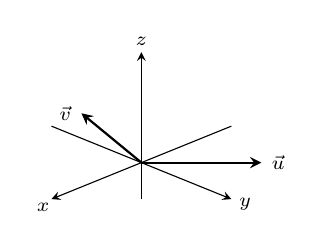
\begin{tikzpicture}[>=stealth]
\begin{axis}[width=175pt,tick label style={font=\scriptsize},axis on top,
axis lines=center,view={135}{35},name=myplot,
xtick=\empty,ytick=\empty,ztick=\empty,
ymin=-1.5,ymax=1.5,xmin=-1.5,xmax=1.5,zmin=-0.5, zmax=1.5,
every axis x label/.style={at={(axis cs:\pgfkeysvalueof{/pgfplots/xmax},0,0)},xshift=-3pt,yshift=-3pt},
xlabel={\scriptsize $x$},
every axis y label/.style={at={(axis cs:0,\pgfkeysvalueof{/pgfplots/ymax},0)},xshift=5pt,yshift=-2pt},
ylabel={\scriptsize $y$},
every axis z label/.style={at={(axis cs:0,0,\pgfkeysvalueof{/pgfplots/zmax})},xshift=0pt,yshift=4pt},
zlabel={\scriptsize $z$}]
\draw [thick,->,draw={\colorone}] (axis cs:0,0,0) -- (axis cs:-1,1,0) node [black,right] {\scriptsize $\vec u$};
\draw [thick,->,draw={\colorone}] (axis cs:0,0,0) -- (axis cs:1,0,1) node [black,left] {\scriptsize $\vec v$};
\end{axis}
\end{tikzpicture}
\end{minipage}}{\mbox{}\\[-\baselineskip]\begin{minipage}[m]{\linewidth}
\centering
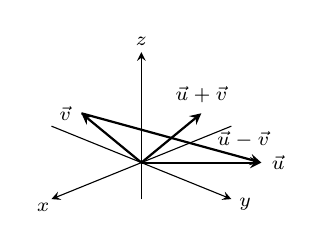
\begin{tikzpicture}[>=stealth]
\begin{axis}[width=175pt,tick label style={font=\scriptsize},axis on top,
axis lines=center,view={135}{35},name=myplot,
xtick=\empty,ytick=\empty,ztick=\empty,
ymin=-1.5,ymax=1.5,xmin=-1.5,xmax=1.5,zmin=-0.5, zmax=1.5,
every axis x label/.style={at={(axis cs:\pgfkeysvalueof{/pgfplots/xmax},0,0)},xshift=-3pt,yshift=-3pt},
xlabel={\scriptsize $x$},
every axis y label/.style={at={(axis cs:0,\pgfkeysvalueof{/pgfplots/ymax},0)},xshift=5pt,yshift=-2pt},
ylabel={\scriptsize $y$},
every axis z label/.style={at={(axis cs:0,0,\pgfkeysvalueof{/pgfplots/zmax})},xshift=0pt,yshift=4pt},
zlabel={\scriptsize $z$}]
\draw [thick,->,draw={\colorone}] (axis cs:0,0,0) -- (axis cs:-1,1,0) node [black,right] {\scriptsize $\vec u$};
\draw [thick,->,draw={\colorone}] (axis cs:0,0,0) -- (axis cs:1,0,1) node [black,left] {\scriptsize $\vec v$};
\draw [thick,->,draw={\colorone}] (axis cs:0,0,0) -- (axis cs:0,1,1) node [black,above] {\scriptsize $\vec u+\vec v$};
\draw [thick,->,draw={\colorone}] (axis cs:1,0,1) -- (axis cs:-1,1,0) node [black,above,pos=.9] {\scriptsize $\vec u-\vec v$};
\end{axis}
\end{tikzpicture}
\end{minipage}}

\exercise{\mbox{}\\[-2\baselineskip]\begin{minipage}[m]{\linewidth}
\centering
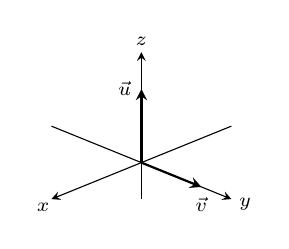
\begin{tikzpicture}[>=stealth]
\begin{axis}[width=175pt,tick label style={font=\scriptsize},axis on top,
axis lines=center,view={135}{35},name=myplot,
xtick=\empty,ytick=\empty,ztick=\empty,
ymin=-1.5,ymax=1.5,xmin=-1.5,xmax=1.5,zmin=-0.5, zmax=1.5,
every axis x label/.style={at={(axis cs:\pgfkeysvalueof{/pgfplots/xmax},0,0)},xshift=-3pt,yshift=-3pt},
xlabel={\scriptsize $x$},
every axis y label/.style={at={(axis cs:0,\pgfkeysvalueof{/pgfplots/ymax},0)},xshift=5pt,yshift=-2pt},
ylabel={\scriptsize $y$},
every axis z label/.style={at={(axis cs:0,0,\pgfkeysvalueof{/pgfplots/zmax})},xshift=0pt,yshift=4pt},
zlabel={\scriptsize $z$}]
\draw [thick,->,draw={\colorone}] (axis cs:0,0,0) -- (axis cs:0,0,1) node [black,left] {\scriptsize $\vec u$};
\draw [thick,->,draw={\colorone}] (axis cs:0,0,0) -- (axis cs:0,1,0) node [black,below] {\scriptsize $\vec v$};
\end{axis}
\end{tikzpicture}
\end{minipage}}{\mbox{}\\[-\baselineskip]\begin{minipage}[m]{\linewidth}
\centering
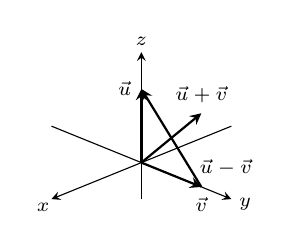
\begin{tikzpicture}[>=stealth]
\begin{axis}[width=175pt,tick label style={font=\scriptsize},axis on top,
axis lines=center,view={135}{35},name=myplot,
xtick=\empty,ytick=\empty,ztick=\empty,
ymin=-1.5,ymax=1.5,xmin=-1.5,xmax=1.5,zmin=-0.5, zmax=1.5,
every axis x label/.style={at={(axis cs:\pgfkeysvalueof{/pgfplots/xmax},0,0)},xshift=-3pt,yshift=-3pt},
xlabel={\scriptsize $x$},
every axis y label/.style={at={(axis cs:0,\pgfkeysvalueof{/pgfplots/ymax},0)},xshift=5pt,yshift=-2pt},
ylabel={\scriptsize $y$},
every axis z label/.style={at={(axis cs:0,0,\pgfkeysvalueof{/pgfplots/zmax})},xshift=0pt,yshift=4pt},
zlabel={\scriptsize $z$}]
\draw [thick,->,draw={\colorone}] (axis cs:0,0,0) -- (axis cs:0,0,1) node [black,left] {\scriptsize $\vec u$};
\draw [thick,->,draw={\colorone}] (axis cs:0,0,0) -- (axis cs:0,1,0) node [black,below] {\scriptsize $\vec v$};
\draw [thick,->,draw={\colorone}] (axis cs:0,0,0) -- (axis cs:0,1,1) node [black,above] {\scriptsize $\vec u+\vec v$};
\draw [thick,->,draw={\colorone}] (axis cs:0,1,0) -- (axis cs:0,0,1) node [black,right,pos=.2] {\scriptsize $\vec u-\vec v$};
\end{axis}
\end{tikzpicture}
\end{minipage}}

}

%\ifthenelse{\boolean{printquestions}}{\pagebreak}{}
\exerciseset{In Exercises}{, find $\norm{\vec u}$, $\norm{\vec v}$, $\norm{\vec u+\vec v}$ and $\norm{\vec u-\vec v}$.}{

\exercise{$\vec u=\bracket{2,1}$,\quad $\vec v =\bracket{3,-2}$}{$\norm{\vec u} = \sqrt{5}$, $\norm{\vec v} = \sqrt{13}$, $\norm{\vec u+\vec v} = \sqrt{26}$, $\norm{\vec u-\vec v} = \sqrt{10}$}

\exercise{$\vec u=\bracket{-3,2,2}$,\quad $\vec v =\bracket{1,-1,1}$}{$\norm{\vec u} = \sqrt{17}$, $\norm{\vec v} = \sqrt{3}$, $\norm{\vec u+\vec v} = \sqrt{14}$, $\norm{\vec u-\vec v} = \sqrt{26}$}

\exercise{$\vec u=\bracket{1,2}$,\quad $\vec v =\bracket{-3,-6}$}{$\norm{\vec u} = \sqrt{5}$, $\norm{\vec v} = 3\sqrt{5}$, $\norm{\vec u+\vec v} = 2\sqrt{5}$, $\norm{\vec u-\vec v} = 4\sqrt{5}$}

\exercise{$\vec u=\bracket{2,-3,6}$,\quad $\vec v =\bracket{10,-15,30}$}{$\norm{\vec u} = 7$, $\norm{\vec v} = 35$, $\norm{\vec u+\vec v} = 42$, $\norm{\vec u-\vec v} = 28$}

}

\exercise{Under what conditions is $\norm{\vec u}+\norm{\vec v} = \norm{\vec u+\vec v}$?
}{When $\vec u$ and $\vec v$ have the same direction. (Note: parallel is not enough.)}

\exerciseset{In Exercises}{, find the unit vector $\vec u$ in the direction of $\vec v$.
}{

\exercise{$\vec v = \la 3,7\ra$
}{$\vec u = \la 3/\sqrt{58},7/\sqrt{58}\ra$
}

\exercise{$\vec v = \la 6,8\ra$
}{$\vec u = \la 0.6,0.8\ra$
}

\exercise{$\vec v = \la 1,-2,2\ra$
}{$\vec u = \la 1/3, -2/3, 2/3\ra$
}

\exercise{$\vec v = \la 2,-2,2\ra$
}{$\vec u = \la 1/\sqrt{3},-1/\sqrt{3},1/\sqrt{3}\ra$
}
}
\exercise{Find the unit vector in the first quadrant of $\mathbb{R}^2$ that makes a $50^\circ$ angle with the $x$-axis.
}{$\vec u = \la \cos 50^\circ,\sin 50^\circ\ra \approx \la 0.643,0.766\ra$.
}

\exercise{Find the unit vector in the second quadrant of $\mathbb{R}^2$ that makes a $30^\circ$ angle with the $y$-axis.
}{$\vec u = \la \cos 120^\circ,\sin 120^\circ\ra = \la -1/2,\sqrt{3}/2\ra$.
}

\exercise{Verify, from Key Idea \ref{idea:unit_vectors}, that $\vec u=\la \sin\theta\cos\varphi,\sin\theta\sin\varphi,\cos\theta\ra$ is a unit vector for all angles $\theta$ and $\varphi$.
}{\begin{align*}
\norm{\vec u} &= \sqrt{\sin^2\theta\cos^2\varphi+\sin^2\theta\sin^2\varphi+\cos^2\theta}\\
						&= \sqrt{\sin^2\theta(\cos^2\varphi+\sin^2\varphi)+\cos^2\theta}\\
						&= \sqrt{\sin^2\theta+\cos^2\theta}\\
						&=1.
\end{align*}
}

\exerciseset{A weight of 100lb is suspended from two chains, making angles with the vertical of $\theta$ and $\varphi$ as shown in the figure below.
\begin{center}
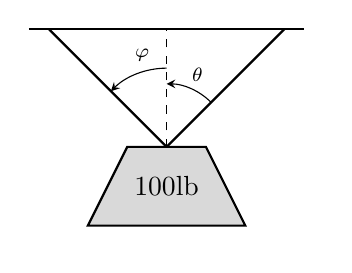
\begin{tikzpicture}
    \filldraw[thick,black,fill=gray!30] (-.5,0) -- (.5,0) -- (1,-1) -- (-1,-1)--cycle;
    \draw (0,-.5) node {100lb};
    \draw [thick] (-1.75,1.5) -- (1.75,1.5);
    \clip (-1.5,1.5) rectangle (2,-1.25);
    \draw [thick,rotate=135] (0,0) -- (3,0);
    \draw [thick,rotate=45] (0,0) -- (3,0);
    \draw [dashed] (0,0) -- (0,2);
    \draw [rotate=45,->,>=stealth] (.8,0) arc (0:45:.8);
    \draw [rotate=67] (1,0) node {\scriptsize $\theta$};
    \draw [rotate=90,->,>=stealth] (1,0) arc (0:45:1);
    \draw [rotate=105] (1.2,0) node {\scriptsize $\varphi$};
\end{tikzpicture}
\end{center}
In Exercises}{,  angles $\theta$ and $\varphi$ are given. Find the force applied to each chain.}{

\exercise{$\theta = 30^\circ$,\quad $\varphi=30^\circ$}{The force on each chain is  $100/\sqrt{3}\approx 57.735$lb.}

\exercise{$\theta = 60^\circ$,\quad $\varphi=60^\circ$}{The force on each chain is  $100$lb.}

\exercise{$\theta = 20^\circ$,\quad $\varphi=15^\circ$}{The force on the chain with angle $\theta$ is approx. $45.124$lb; the force on the chain with angle $\varphi$ is approx. $59.629$lb.}

\exercise{$\theta = 0^\circ$,\quad $\varphi=0^\circ$}{The force on each chain is 50lb.}

}

\exerciseset{A weight of $p$lb is suspended from a chain of length $\ell$ while a constant force of $\vec F_w$ pushes the weight to the right, making an angle of $\theta$ with the vertical, as shown in the figure below. 
\begin{center}
\myincludegraphics{figures/fig10_02_exset_06}
\end{center}
In Exercises}{,  a force $\vec F_w$ and length $\ell$ are given. Find the angle $\theta$ and the height the weight is lifted as it moves to the right.
}{

\exercise{$\vec F_w=1$lb, \quad $\ell = 1$ft, \quad $p = 1$lb
}{$\theta = 45^\circ$; the weight is lifted $0.29$ ft (about 3.5in).
}

\exercise{$\vec F_w=1$lb, \quad $\ell = 1$ft, \quad $p = 10$lb
}{$\theta = 5.71^\circ$; the weight is lifted $0.005$ ft (about 1/16th of an inch).
}

\exercise{$\vec F_w=1$lb, \quad $\ell = 10$ft, \quad $p = 1$lb
}{$\theta = 45^\circ$; the weight is lifted $2.93$ ft.
}

\exercise{$\vec F_w=10$lb, \quad $\ell = 10$ft, \quad $p = 1$lb
}{$\theta = 84.29^\circ$; the weight is lifted $9$ ft.
}
}